\documentclass[12pt,a4paper]{article}
\usepackage{huy}
\pagestyle{empty}
\usepackage[margin=2cm]{geometry}
\begin{document}
\intro{DATABASE}{Subqueries}
\section{Subqueries}
A subquery is a complete SELECT statement embedded within another SELECT statement. The results of this \emph{inner} SELECT statement  (or \emph{subselect}) are used in the outer statement to help determine the contents of the final results. A subselect can be used in the WHERE and HAVING clauses of an outer SELECT statement, where it is called a \emph{subquery} or \emph{nested query}. There are three types of subquery:
\begin{itemize}
\item A \emph{scalar subquery} returns a single column and a single row, that is, a single value (Listing \ref{scalar-subquery}).
\item A \emph{row subquery} returns multiple columns, but only a single row.
\item A \emph{table subquery} returns multiple columns and multiple rows. A table subquery can be used as an operand for the IN predicate.
\end{itemize}
\begin{listing}
\begin{lstlisting}[language=sql,style=cool]
SELECT staffNo, fName, lName, position
FROM Staff
WHERE branchNo =(SELECT branchNo
     		FROM Branch
     		WHERE street = '163 Main St' );
\end{lstlisting}
\caption{A scalar subquery}\label{scalar-subquery}
\end{listing}
We can think of the subquery as producing a temporary table with results that can be accessed and used by the outer statement. The subquery itself is always enclosed in parentheses.
\section{Practical part}
\begin{enumerate}
\item Show the branch where Ann works as well as the Street and City
of that Branch.
\database{1-Ann-branch.sql}
%\begin{figure}[hbtp]
%	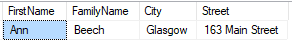
\includegraphics[scale=1]{1-Ann-branch.PNG}
%	\end{figure}
\item Show any Staff who works in the branch at ’32 Manse Road’ and only those
whose position is ‘Assistant’ in that same branch.
\database{2-branch-position.sql}
%\begin{figure}[hbtp]
%	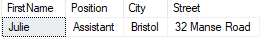
\includegraphics[scale=1]{2-branch-position.PNG}
%	\end{figure}
\item Show the owner of the property for rent at address ‘Slippery Lane 16’.
\database{3-owner-street.sql}
%\begin{figure}[hbtp]
%	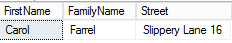
\includegraphics[scale=1]{3-owner-street.PNG}
%	\end{figure}
\item List the names of all clients who have viewed a property at 15th of June.
\database{4-viewdate.sql}
%\begin{figure}[hbtp]
%	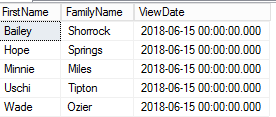
\includegraphics[scale=1]{4-viewdate.PNG}
%	\end{figure}
\item List the names of all clients who have viewed a property at 15th of June or
at 16th of June.
\database{5-2viewdate.sql}
%\begin{figure}[hbtp]
%	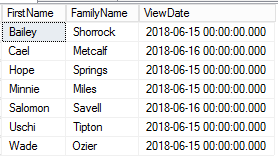
\includegraphics[scale=1]{5-2viewdate.PNG}
%	\end{figure}
\item List the name of all clients who has viewed a property at 15th of June and
who did not give any comments.
\database{6-null-comment.sql}
%\begin{figure}[hbtp]
%	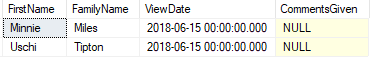
\includegraphics[scale=1]{6-null-comment.PNG}
%	\end{figure}
\item Show the name of a staff member who manages property for rent at ‘8
Naval Drive’.
\database{7-staff-street.sql}
%\begin{figure}[hbtp]
%	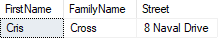
\includegraphics[scale=1]{7-staff-street.PNG}
%	\end{figure}
\item Find the names of all clients who have viewed Flats.
\database{8-view-flat.sql}
%\begin{figure}[hbtp]
%	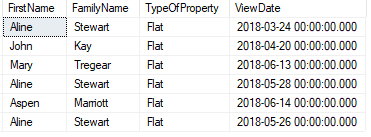
\includegraphics[scale=1]{8-view-flat.PNG}
%	\end{figure}
\end{enumerate}	
\end{document}
